\chapter{A Framework for the Reinforcement Learning of Decision Tree Policies}
\section{Learning Decision Tree policies}
Deicision tree policies offer transparency over neural network policies (cite). 
One can attribute an importance measure to each feature of the state for the deicison of a tree policy which is harder to do for neural networks (cite).

Recently, algorithms have been developed to return decision tree policies for an MDP.
Those algorithms, like any interpretable machine learning method, are either direct or indrect (cite).
We propose an additional distinction amongst the direct methods: algorithms learning parametric trees and algorithms learning non-parametric trees.

Parametric trees are not ``grown'' from the root by iteratively adding internal or leaf nodes depending on the interpretability-performance trade-off to optimize, but are rather ``optimized'': the depth, internal nodes arrengement, and state-features to consider in each nodes are fixed \textit{a priori} and only the tested thresholds of each nodes are optimized similarly to how the weights of a neural network are optimized.
As the reader might have guessed, those parametric trees are advantageous in that they can be learned with gradient descent and in the context of decision tree policies, with the policy gradient (cite).
The downside of those approaches is that a user cannot know \textit{a priori}  what a ``good'' tree policy structure should be for a particular MDP: either the specified structure is too deep and pruning will be required after training or the tree structure is not expressive enough to encode a good policy. 
Similar approaches exist in supervised learning exist where a parametric tree is fitted with gradient descent (cite) GRADTREE and the work of the authors in KDD. However their benefit over non-parametric trees have not been shown.
When parametric trees are learned for MDPs (cite); extra stabilizing tricks are required during training such as adaptive batch sizes.

Non-parametric trees are the standard model in supervised learning (cite) and can naturally trade-off between interpretability and performances. However, specialized approaches are required since growing a tree from the root in an RL fashion is not possible.
In the next section we present, to the best of our knowledge, the only direct approach to learn non-parametric decision tree policies for MDPs; Iterative Bounding MDPs (cite). 

Other more specialized approaches deal with tree policies either for specific MDPs like maze (cite) or for very small depth (cite) or when the MDP model is known (cite)
\section{Iterative Bounding Markov Decision Processes}
In 2021, Topin et. al. introduced Iterative Bouding Markov Decision Processes (IBMDPs) with the promise of sticking the challenges of non-parametric decision tree policy learning in the problem formulation rather than in the learning algorithms.
Given a base MDP for which one wants to learn a decision tree policy, IBMDPs are an augmented version of this base MDP with more state features, more actions, additinal reward signal, and additional transition kernel.
Then author showed that certain IBMDP policies, that can be learned with RL, are equivalent to decision tree policies for the base MDP. 
\section{Litterature and results on POMDPs}
CITE ALL NAMES OF THIS PARTICULAR POMDP (c.f. Olivier Buffet)

\section{IBMDP and Didactic example}
Given an MDP $\mathcal{M}= \langle S, A, R, T, T_0 \rangle$, an Iterative Bounding Markov decision process is defined as follows.
\begin{definition}
    Given an MDP $\mathcal{M}= \langle S, A, R, T, T_0 \rangle$, an Iterative Bounding Markov decision process $\mathcal{M}_{IB}$ is a tuble $\langle S, O, A, A_{IG}, R, \zeta, T, T_0, P\rangle$.
    The IBMDP is an augmented version of an MDP. The states in an IBMPD are concatenations of $s\in S \subset [L_1, U_1]\times\dots \times [L_n, U_n] \subsetneq \mathbb{R}^n$ and bounding values $o = (L_0) \in O$ 
\end{definition}

\begin{algorithm}[t]
    \KwData{IBMDP policy $\pi$ and observation $obs$}
    \KwResult{Decision tree policy extracted from $\pi$}
    
    \SetKwProg{Fn}{Function}{:}{}
    \SetKwFunction{SubtreeFromPolicy}{Subtree\_From\_Policy}
    
    \Fn{\SubtreeFromPolicy{$obs, \pi$}}{
        $a \leftarrow \pi(obs)$ \\
        \If{$a \in A_b$}{
            \Return Leaf\_Node(action: $a$) \Comment{// Leaf if base action}
        }
        \Else{
            $(c, v) \leftarrow a$ \Comment{// Splitting action is feature and value} \\
            $v_p \leftarrow v \times (obs[c^h] - obs[c^l]) + obs[c^l]$ \\
            $obs_L \leftarrow obs; \quad obs_R \leftarrow obs$ \\
            $obs_L[c^h] \leftarrow v_p; \quad obs_R[c^l] \leftarrow v_p$ \\
            $child_L \leftarrow$ Subtree\_From\_Policy$(obs_L, \pi)$ \\
            $child_R \leftarrow$ Subtree\_From\_Policy$(obs_R, \pi)$ \\
            \Return Internal\_Node(feature: $c$, value: $v_p$, children: $(child_L, child_R)$)
        }
    }
    
    \Return Subtree\_From\_Policy$(obs, \pi)$
    \caption{Extract a Decision Tree Policy from an IBMDP policy $\pi$, beginning traversal from $obs$.}\label{alg_extract_tree}
\end{algorithm}

\begin{figure}[ht]
    \centering
    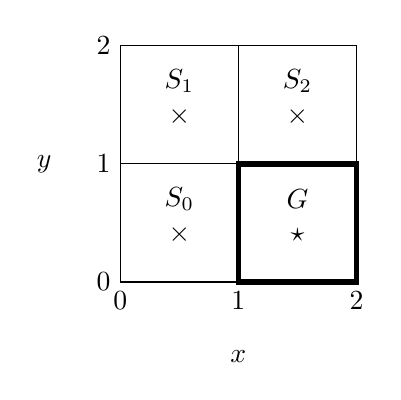
\begin{tikzpicture}[scale=1.5]
        % Draw the grid cells
        \draw (0,0) grid (2,2);
        
        % Add ticks on axes
        \foreach \x in {0,1,2}
            \node[below] at (\x,0) {$\x$};
        \foreach \y in {0,1,2}
            \node[left] at (0,\y) {$\y$};
        
        \node[left] at (-0.5, 1) {$y$};
        \node[below] at (1, -0.5) {$x$};
        
        % Label cells
        \node at (0.5,0.7) {$S_0$};
        \node at (0.5,0.4) {$\times$};
    
        \node at (0.5,1.7) {$S_1$};
        \node at (0.5,1.4) {$\times$};
    
        \node at (1.5,1.7) {$S_2$};
        \node at (1.5,1.4) {$\times$};
    
        
        % Goal state in bottom right with double border
        \draw[line width=2pt] (1,0) rectangle (2,1);
        \node at (1.5,0.7) {$G$};
        \node at (1.5,0.4) {$\star$};
    
        
    \end{tikzpicture}
    \caption{The 2×2 grid world environment with states $S_0$, $S_1$, $S_2$, and goal state $G$.}\label{fig:grid-world}
    \end{figure}
In the next chapter we show the limitation of both direct and indirect approaches for this problem.


